 \documentclass[book.tex]{subfiles}
\begin{document}

\section{Building layer for layer}
Each tile on the screen can contain up to three layers: the background tile, the foreground tile, and a sprite layer. It requires multiple redrawing on the same tile:
\begin{enumerate}
  \item Draw the background tile or a combined background and foreground tile.
  \item Draw the sprites.
  \item Re-draw the foreground tile if the sprite should not appear on top.
\end{enumerate}

\par
In the best case, the engine must read and write 128 bytes (2 * 16 bytes * 4 memory banks) to VRAM for a background tile only. In the worst case, up to 512 bytes are needed (background, foreground, sprite, and foreground again), with several bitwise operations involved. For the sake of speed, all code is written in assembly, as explained in the following sections.

\subsection{Draw background and foreground tiles}
Drawing the background tiles is straightforward, as it only involves copying 128 bytes to VRAM. However, drawing foreground tiles on top of the background requires an additional mask layer, which defines which pixels are overwritten by the foreground tile. \\

\begin{figure}[H]
\centering
 \begin{subfigure}{0.32\textwidth}
 	\centering
 	\includegraphics[width=0.7\textwidth]{screenshots_300dpi/game/mask_tiles_1.png}
 	\caption{Background tile.}
 \end{subfigure}
 \begin{subfigure}{0.32\textwidth}
 	\centering
 	\includegraphics[width=0.7\textwidth]{screenshots_300dpi/game/mask_tiles_2.png}
 	\caption{\cw{AND} foreground mask.}
 \end{subfigure}
 \begin{subfigure}{0.32\textwidth}
 	\centering
 	\includegraphics[width=0.7\textwidth]{screenshots_300dpi/game/mask_tiles_3.png}
 	\caption{\cw{OR} foreground bitmap.}
 \end{subfigure}

\caption{Merge foreground with background tile.}
\label{fig:foreground_tile}
\end{figure}

Combining the background and foreground tile is handled by the \cw{RFL\_NewTile} function, using the \cw{AND} bitwise operator to clear the background and the \cw{OR} bitwise operator to write the foreground tile.\\

\par
\begin{minipage}{\textwidth}
  \lstinputlisting[language={[x86masm]Assembler}]{code/update_tile.asm}
  \end{minipage}
  \label{update_tile}


\subsection{Drawing sprites}
The next step is to render sprites on the screen. Most home computers of that era had built-in sprite functionality on the video card. For example, on a MSX computer, one could simply enter\\

\par
\begin{minipage}{\textwidth}
  \lstinputlisting[language=C]{code/msx_sprite.c}
  \end{minipage}
  \label{msx_sprite}

\par
to display a sprite on the screen. Updating the \cw{(X, Y)} coordinates would move the sprite, with the display adapter handling everything else. However, the concept of sprites did not exist on EGA cards, so game developers had to implement their own solution.\\

\par
A challenge arises from the fact that sprites can move freely across the screen and are not byte-aligned. To address this, the bit-shifting technique described in section \ref{section:bitshifting} is used. When caching a sprite into memory, each sprite is copied four times, with each copy shifted by two or more pixels using this technique. The property \cw{*spr->shifts} determines the number of bit shifts applied to each of the four copies.\\


\begin{figure}[H]
  \centering
  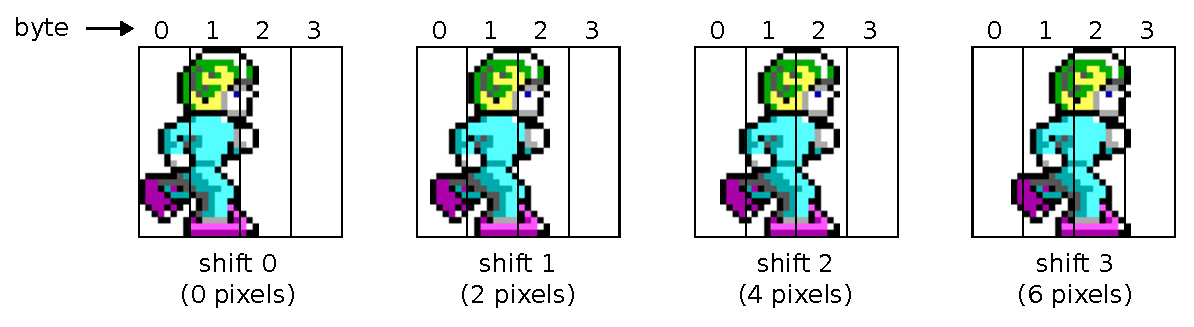
\includegraphics[width=\textwidth]{imgs/drawings/sprite_shift.eps}
  \caption{Sprite shifted in 4 steps.}
  \label{fig:sprite_shift}  
\end{figure}

\par
Displaying the correct shifted sprite is as simple as\\
\par
\begin{minipage}{\textwidth}
  \lstinputlisting[language=C]{code/sprite_shift.c}
  \end{minipage}
  \label{sprite_shift}  

\par
\begin{minipage}{\textwidth}
  \lstinputlisting[language=C]{code/shift_sprite.c}
  \end{minipage}
  \label{shift_sprite}
  

\par
If multiple sprites are displayed on the same tile, each sprite is assigned a priority from 0 to 3 to determine the drawing order. A sprite with a higher priority number is always drawn on top of sprites with a lower priority. Since sprites are always drawn on top of tiles, this can create unnatural situations, such as when Commander Keen is climbing through a hole, as illustrated in Figure \ref{fig:draw_layers}.\\

\begin{figure}[H]
\begin{subfigure}{.25\textwidth}
  \centering
  \includegraphics[width=.9\textwidth]{screenshots_300dpi/game/tile_composite_1.png}
  \caption{Background tile.}
\end{subfigure}%
\begin{subfigure}{.25\textwidth}
  \centering
  \includegraphics[width=.9\textwidth]{screenshots_300dpi/game/tile_composite_2.png}
  \caption{Foreground tile.}
\end{subfigure}
\begin{subfigure}{.25\textwidth}
  \centering
  \includegraphics[width=.9\textwidth]{screenshots_300dpi/game/tile_composite_3.png}
  \caption{Sprite on top.}
\end{subfigure}
\caption{Unnatural situation where Commander Keen is in front of a hole.}
\label{fig:draw_layers}
\end{figure}

\par
To draw sprites 'inside' a foreground tile, a small trick is used by introducing a priority foreground tile. As explained in section \ref{section:foreground_tile_info}, each foreground tile is enriched with INTILE ("inside tile") information. If the highest bit (\cw{80h}) of INTILE is set, that foreground tile has a higher priority than sprites with priority 0, 1, or 2. Therefore, the following drawing order is applied:

\begin{enumerate}
  \item Draw the background tile and the masked foreground tile.
  \item Draw sprites with priority 0, 1, and 2 (in that order), and mark the corresponding tile in the tile buffer array with a '3', as illustrated in Figure \ref{fig:kc1_3_tile_update_sprite} on page \pageref{fig:kc1_3_tile_update_sprite}.
  \item Scan the tile buffer array for tiles marked with '3'. If the corresponding foreground INTILE high bit (\cw{80h}) is set, redraw the masked foreground tile.
  \item Finally, draw sprites with priority 3. These sprites are always drawn on top of everything.
\end{enumerate}
\par
The priority foreground tiles are updated in the \cw{RFL\_MaskForegroundTiles()} function.\\

\begin{figure}[H]
\centering
\begin{subfigure}[t]{.245\textwidth}
  \centering
  \includegraphics[width=.9\textwidth]{screenshots_300dpi/game/tile_composite_1.png}
  \caption{Background tile.}
\end{subfigure}%
\begin{subfigure}[t]{.245\textwidth}
  \centering
  \includegraphics[width=.9\textwidth]{screenshots_300dpi/game/tile_composite_2.png}
  \caption{Foreground tile.}
\end{subfigure}
\begin{subfigure}[t]{.245\textwidth}
  \centering
  \includegraphics[width=.9\textwidth]{screenshots_300dpi/game/tile_composite_3.png}
  \caption{Sprite on top.}
\end{subfigure}
\begin{subfigure}[t]{.245\textwidth}
  \centering
  \includegraphics[width=.9\textwidth]{screenshots_300dpi/game/tile_composite_4.png}
  \caption{Redraw masked foreground tile.}
\end{subfigure}
\caption{Draw sprite inside a tile, by redrawing foreground tile.}
\label{fig:clip_tinf}
\end{figure}

\par
\begin{minipage}{\textwidth}
  \lstinputlisting[language={[x86masm]Assembler}]{code/mask_foreground_tile.asm}
\end{minipage}
\label{mask_foreground_tile}
\par

\end{document}